\section{Экспериментальная установка}

\subsection{Коллайдер KEK}
Ускоритель KEKB является электрон-позитронным коллайдером, состоящим из двух 
колец, пересекающихся в одной точке под углом $22\,\text{mrad}$, что позволяет измерять CP-асимметрию. 
Пучки электронов и позитронов сталкиваются с энергией $8\,\text{GeV}$ и $3.5\,\text{GeV}$ соответственно.
Пучки рождаются на фотонной фабрике и, проходя через линейный ускоритель, где разгоняются до скорости, близкой к скорости света, 
передаются в основные кольца. В режиме накопления пучка подача происходит непрерывно, а в нормальном режиме 
сбора данных - периодически, раз в несколько миллисекунд.

Основной целью было производство большого количества B-мезонов. Работа ускорителя началась в декабре
1998 года и закончилась в конце июня 2010 года. За это время KEKB установил мировой
рекорд по светимости - $2.11\times 10^{34} cm^{-2}s^{-1}$, который на сегодняшний день был
превзойдён только на коллайдере SuperKEKB - усовершенствованной версии, собранной
на основе KEKB. За все время было собрано $825.547fb^{-1}$.

\begin{figure}[H]
    \centering
    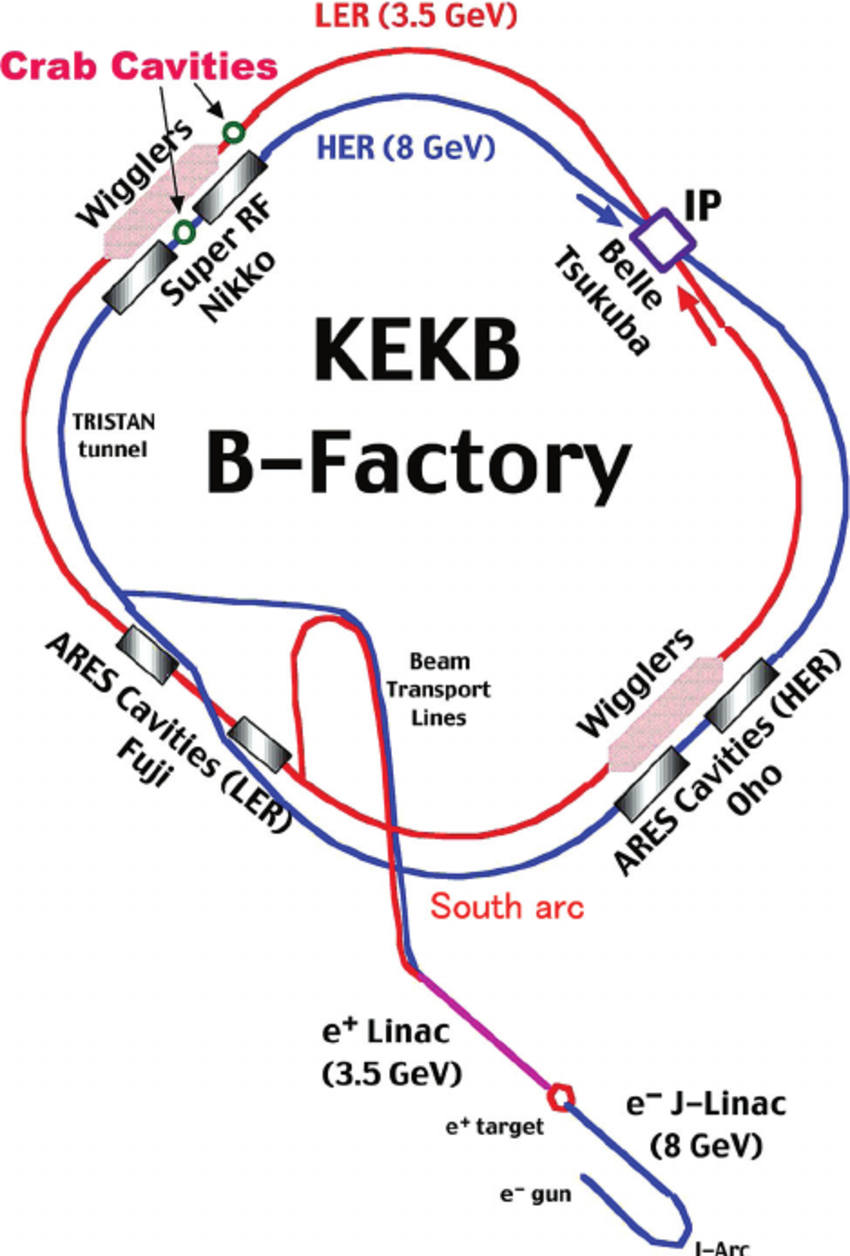
\includegraphics[width=0.5\linewidth]{img/kekb.png}
    \caption{Ускорительный комплекс KEKB}
    \label{the:kek}
\end{figure}

\subsection{Детектор Belle}

Детектор Belle охватывал весь азимутальный угол, а также перекрывал 
часть полярного угла от $17^{\circ} $ до $150^{\circ} $, что соответствует $0.74$
полного телесного угла. Установка окружала точку взаимодействия и состояла 
из вершинного кремниевого детектора (SVD), центральной дрейфовой 
камеры (CDC) из 50 цилиндрических слоёв, массива аэрогелевых черенковских 
счётчиков (ACC), системы измерения времени пролёта (TOF) из сцинтилляционных 
счётчиков, электромагнитного калориметра (ECL), изготовленного из кристалов 
йодида цезия (CsI), и переднего калориметра (EFC), расположенных внутри 
сверхпроводящего соленоида, обеспечивающего магнитное поле величиной 
$1.5 Tl$. В железном ярме электромагнита был расположен детектор $K_L^0$ мезонов 
и $\mu$ (KLM), составленный из стеклянных резистивных плоских камер. 
Общий вид детектора Belle показан на рис. \ref{the:belle}.
\begin{figure}[H]
    \centering
    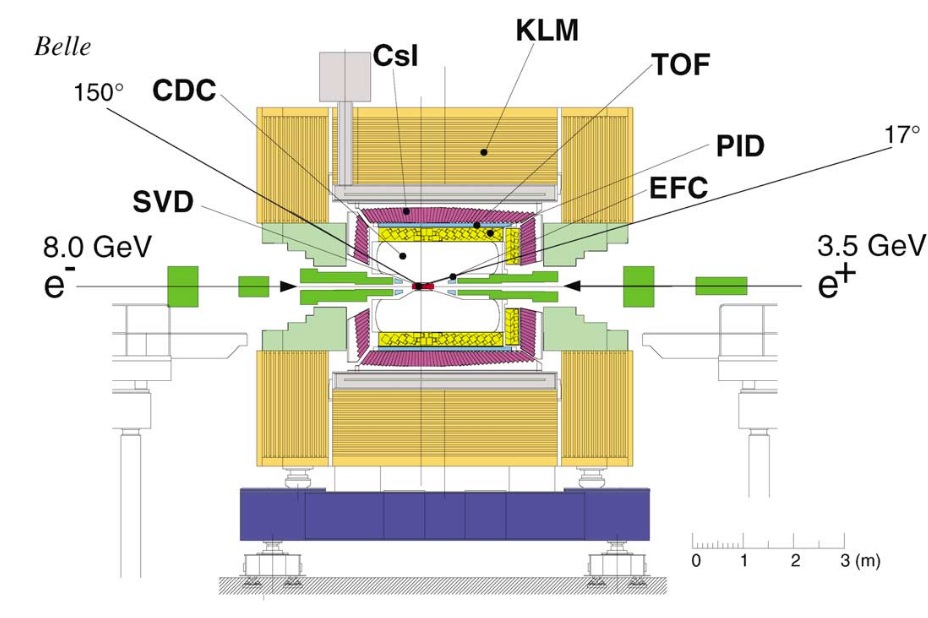
\includegraphics[width=0.8\linewidth]{img/the_belle.png}
    \caption{Декткор Belle в сечении}
    \label{the:belle}
\end{figure}



